

\documentclass[10pt]{article}

\usepackage[swedish]{babel}
\usepackage[utf8]{inputenc}
\usepackage{times}
\usepackage{mathptmx}  
\usepackage{pdfpages}
\usepackage{mcode}
\usepackage{appendix}
\usepackage[margin={2.5cm,2.5cm}]{geometry}
\usepackage{multicol}

\raggedbottom
\sloppy

\newcommand{\todo}[1]{\textbf{\textcolor{red}{#1}}}

\title{Laborationsrapport i TSKS10 \emph{Signaler, Information och Kommunikation}}

\author{Alexander Yngve\\aleyn573, 930320-6651}

\date{8 maj, 2015}

\begin{document}

% Framsida
\maketitle

\clearpage

% Brödtext
\begin{multicols}{2}
\section{Inledning} \label{inledning}

Målet med den här laborationen var att demodulera en smalbandig I/Q-modulerad signal skickad från en tänkt radiostation och lyssna på dess innehåll. Signalens innehåll består av musikaliska melodier, ordspråk och vitt brus. En del av uppgiften var att identifiera ordspråken. Förutom demodulering skulle även signalens bärfrekvens bestämmas samt ekoeffekter tas hänsyn till. Resultatet av laborationen blev kända värden på signalens bärfrekvens, ekotidsfördröjning samt en användbar signal där ordspråken kunde höras.

Från labbhandledningen fås följande information om signalen:

\begin{itemize}
\item Radiostationen sänder ut signalen $x(t) = x_I(t)cos(2\pi f_ct) - x_Q(t)sin(2\pi f_ct) + z(t)$, där $f_c$ är signalens bärfrekvens och $z(t)$ är andra signaler ämnade åt någon annan. $x_I$ och $x_Q$ är de intressanta signalerna med relevant innehåll.
\item På grund av ekoeffekter i radioutbredningsmiljön så tar vi emot signalen $y(t) = x(t - \tau_1) + 0.9x(t - \tau_2)$. 
\item Bärfrekvensen $f_c$ är en multipel av 19 kHz.
\item Den mottagna signalen lågpassfiltreras och samplas sedan med en frekvens på $f_s = 400000$ Hz.
\end{itemize}

\section{Metod}

Laborationen kan delas in i tre deluppgifter, bestämming av bärfrekvens samt filtrering i smalbandet, bestämning av ekots tidsfördröjning samt filtrering av detta och slutligen I/Q-demodulering. MATLAB användes som verktyg för att behandla signalen.

\subsection{Bärfrekvens och filtrering} \label{filtrering}
Bärfrekvensen $f_c$ fås med hjälp av fouriertransformen $Y(f)$ till signalen $y(t)$. Figur \ref{amplitudspektrum} visar amplitudspektrumet $|Y(f)|$. Ur figuren fås att det finns innehåll i närheten av tre olika bärfrekvenser. De frekvenser som matchar kritieriet att vara en multipel av 19 kHz är våra möjliga bärfrekvenser.

\begin{itemize}
\item Signal $y_1$ med $f_{c1}=38$ kHz
\item Signal $y_2$ med $f_{c2}=76$ kHz
\item Signal $y_3$ med $f_{c3}=114$ kHz
\end{itemize}

Signalerna på de olika frekvenserna filtreras ut med hjälp av ett bandpassfilter med övre respektive undre gräns $f_{ci} - B/2$ och $f_{ci} + B/2$ där $i = 1,2,3$. Då vi vet att signalen ska innehålla hörbart ljud väljs bandbredden $B=20000$ Hz.


Figur \ref{signaler} visar de filtrerade smalbandssignalerna i tidsdomänen. Signalerna $y_1$ och $y_2$ med bärfrekvens $f_{c1}$ och $f_{c2}$ ser ut att vara rent brus eller snarlikt. Signalen $y_3$ med bärfrekvens $f_{c3}$ ser däremot ut att ha korrekt innehåll, två delar som skulle kunna vara toner och tal och en avslutande del brus.

\subsection{Hantering av eko} \label{eko}
För att få bort ekoeffekterna i signalen måste vi först veta ekots tidsfördröjning. Detta görs genom en autokorrelation på signalen. Signalen $y_2$ som bara innehåller brus används då denna typ av vågform ger ett tydligare resultat enligt kursboken. I figur \ref{xcorr} syns huvudtoppen vid tiden $t = 0$ och sidotoppen vid $t = 0.430$, alltså är ekots tidsfördröjning $\tau = \tau_{1} - \tau_{2} = 0.430$ sekunder.

Med en känd tidsfördröjning samt amplitud på ekot från avsnitt \ref{inledning} kan nu den ekofria signalen $y_{3}^{'}$ tas fram från $y_3$. Detta görs genom $y_{3}^{'}(t) = y_{3}(t) - 0.9y_{3}^{'}(t - \tau)$ för alla $t > \tau$. Då det är uppenbart att det inte finns något eko för $0 \leq t \leq \tau$ gäller $y_{3}^{'}(t) = y_{3}(t)$ i det intervallet.

Implementationen i MATLAB utför ekodämpningen på ett helt block av sampel i taget istället för en och en. Detta för att få en snabbare exekveringstid, i övrigt är det samma algoritm. Blockets storlek är antalet sampel som motsvarar $\tau = 0.430$ sekunder, det vill säga $f_s\tau = 172000$ sampel.

\subsection{I/Q-demodulering}
Nu återstår endast demodulering innan signalen kan spelas upp som hörbart ljud. Från kursboken har vi givet $x_I(t) = \mathcal{H}_{B/2}^{LP}\{2x(t)cos(2\pi f_ct)\}$ och $x_Q(t) = -\mathcal{H}_{B/2}^{LP}\{2x(t)sin(2\pi f_ct)\}$, där i vårt fall $x(t) = y_{3}^{'}(t)$ enligt avsnitt \ref{eko}, $f_c = f_{c3} = 114000$ Hz och $B = 20000$ Hz enligt avsnitt \ref{filtrering}. Basbandssignalerna $x_I$ och $x_Q$ innehåller nu hörbart ljud som kan spelas upp i valfri mediaspelare!

\section{Resultat}

Den sökta informationen är:

\begin{itemize}
\item Bärfrekvensen för nyttosignalen är $f_c = 114000$ Hz.
\item Differensen $\tau_{2} - \tau_{1} = 0.430$ s.
\item Ordspråket i I-signalen är ''även den mest skröpliga mussla kan innehålla en pärla''.
\item Ordspråket i Q-signalen är ''skrattar bäst som skrattar sist''.
\end{itemize}
\end{multicols}

\clearpage

\begin{figure}
  \centering
  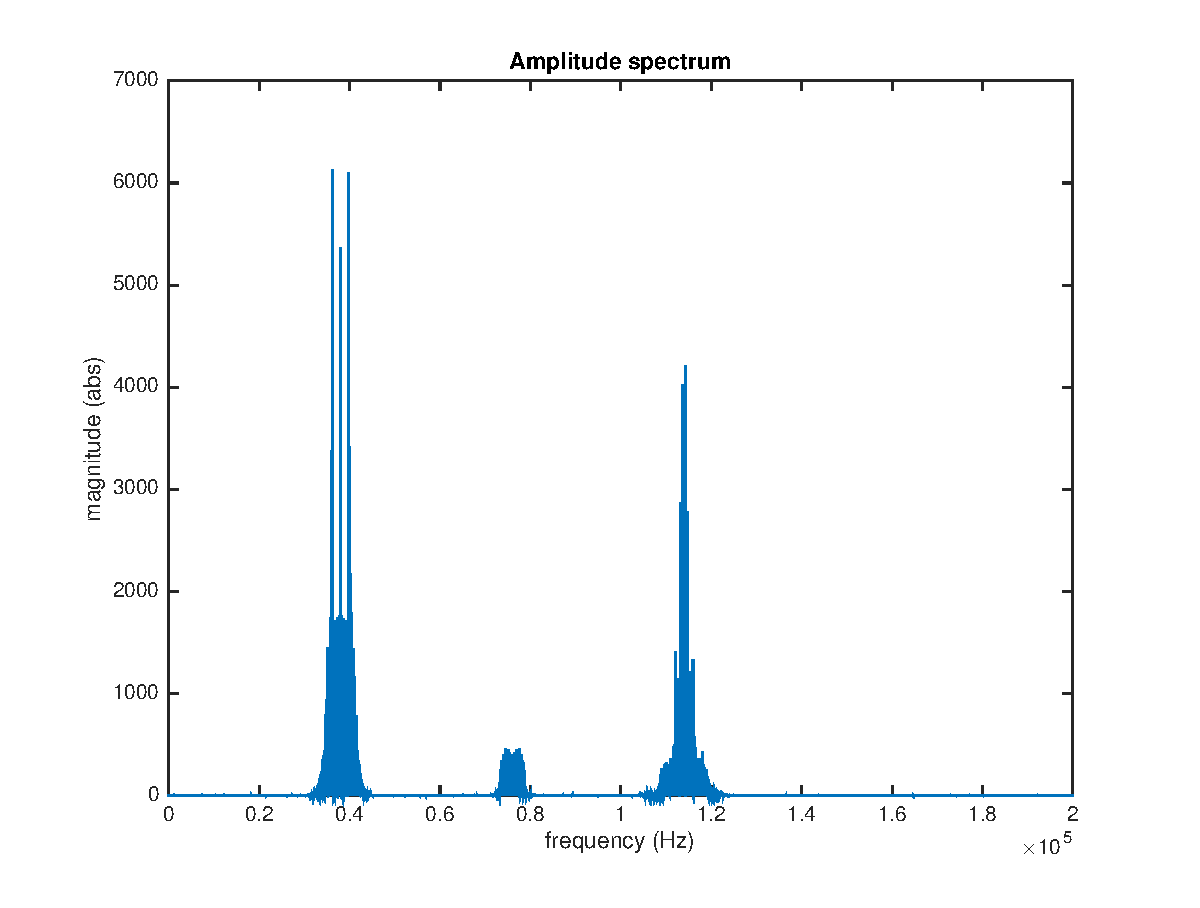
\includegraphics[scale=0.55]{figurer/amplitudspektrum.eps}
  \caption{Amplitudspektrum}
  \label{amplitudspektrum}
\end{figure}

\begin{figure}
  \centering
  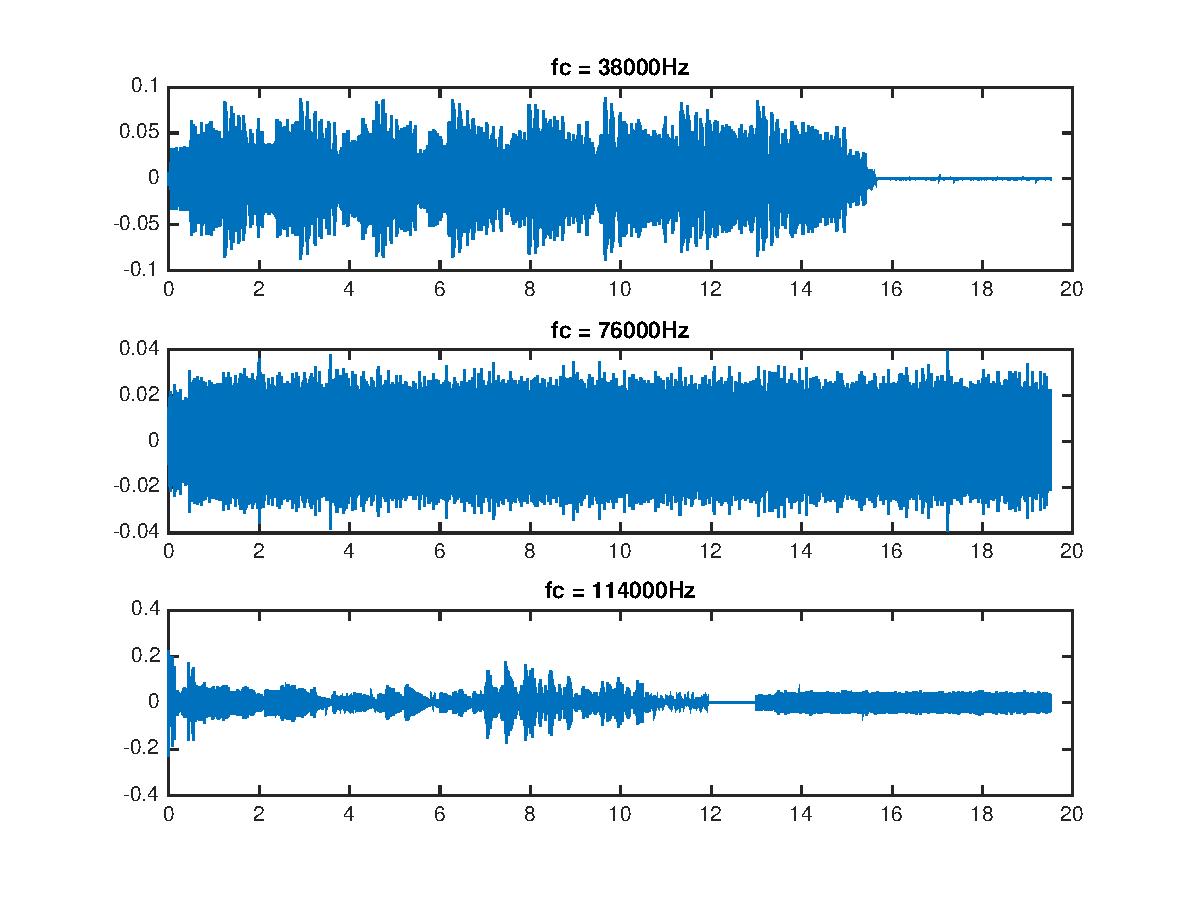
\includegraphics[scale=0.55]{figurer/signaler.eps}
  \caption{Radiostationens tre signaler i tidsdomänen}
  \label{signaler}
\end{figure}

\begin{figure}
  \centering
  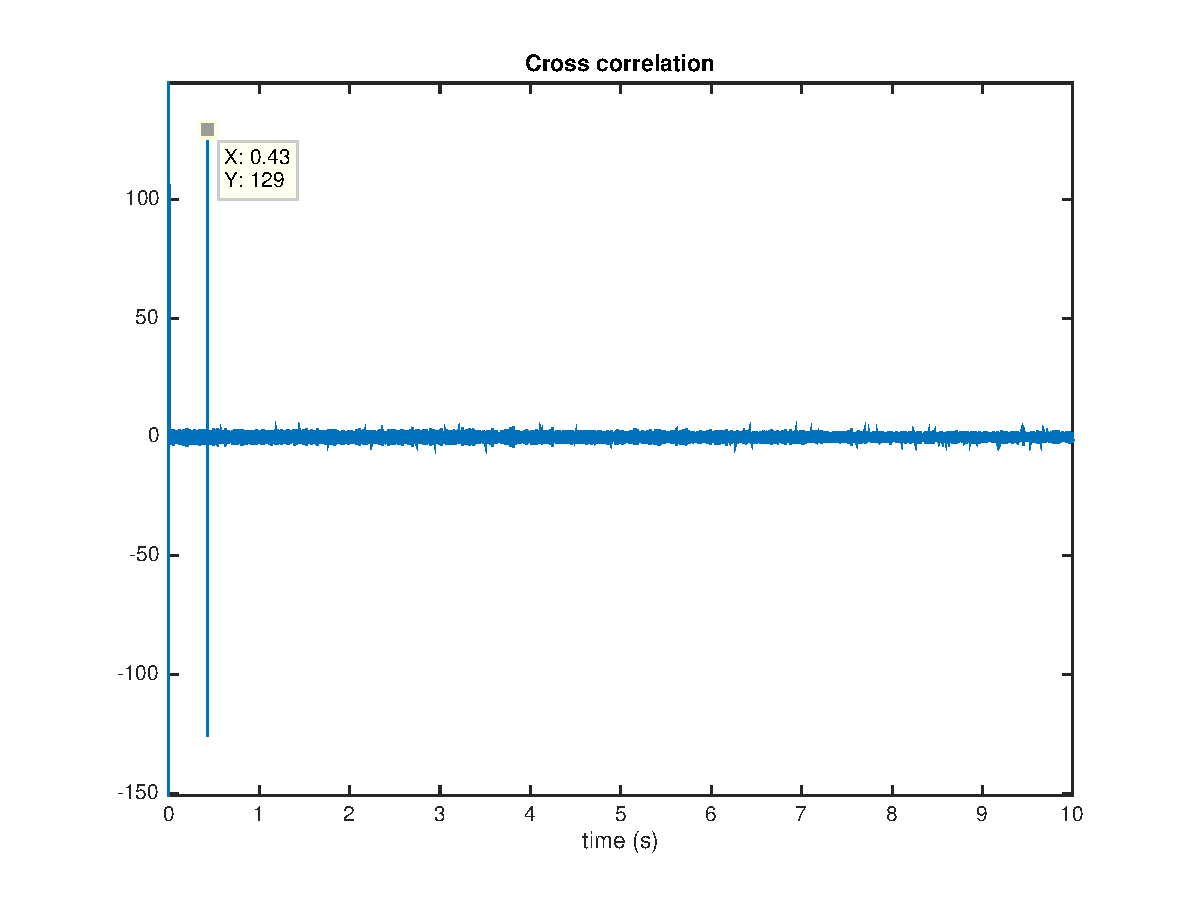
\includegraphics[scale=0.55]{figurer/xcorr.eps}
  \caption{Autokorrelation för att bestämma ekots tidsfördröjning}
  \label{xcorr}
\end{figure}

\clearpage

% Programkod
\begin{multicols}{2}
\begin{appendices}
\section{Programkod}
\lstinputlisting[breaklines=true]{../matlab/lab.m}
\end{appendices}
\end{multicols}

\end{document}
